\documentclass{article}
\usepackage{amsmath,  amsthm,  amssymb,  bm,  graphicx, mathrsfs, ctex, caption, subfigure, multicol, multienum, bm}
\usepackage[hidelinks]{hyperref}
\usepackage{anyfontsize}
\usepackage{xeCJK}

\usepackage{geometry}
\geometry{a5paper, scale=0.8}

\newtheorem*{note}{注}
\newtheorem*{solution}{解}
\newtheorem{theorem}{定理}[section]
\newtheorem{definition}[theorem]{定义}
\newtheorem{lemma}[theorem]{引理}
\newtheorem{corollary}[theorem]{推论}
\newtheorem{example}[theorem]{例}
\newtheorem{proposition}[theorem]{命题}


\begin{document}

\begin{center}
    \huge\bf review
\end{center}

\section{Preliminary}
\begin{enumerate}
    \item Sets and Indices:
    \begin{itemize}
        \item 
        \item 
    \end{itemize}
    \item Variables:

    \item Parameters:

\end{enumerate}

\section{Benders Decomposition}
\subsection{Unified Primal Subproblems for Benders Decomposition}
\begin{figure}[htbp]
    \centering
    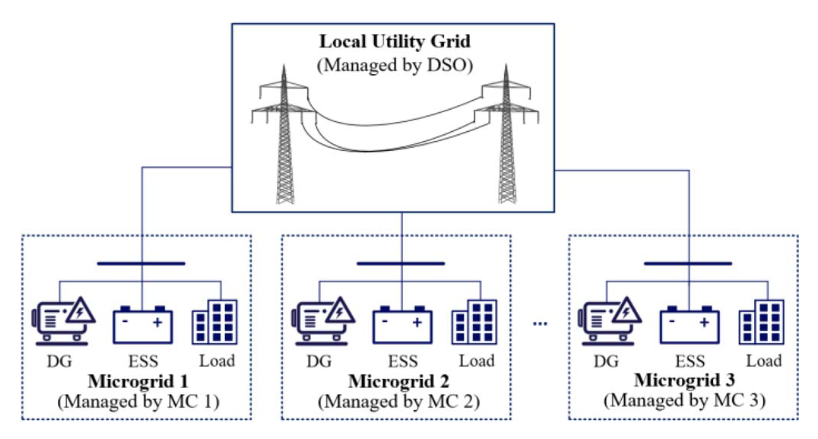
\includegraphics[width=0.8\textwidth]{./pic/NetworkedStructure.png}
    \caption{系统结构示意图}
    \label{fig:structure}
\end{figure}

为了表示方便, 将原始模型以矩阵形式重新表示为如下模型:
\begin{subequations}
    \begin{align}
        \min_{x, y, z}\quad &\mathbf{a}^\mathrm{T}\mathbf{x}+\sum_i\mathbf{b}_i^\mathrm{T}\mathbf{y}_i+\sum_i\mathbf{c}_i^\mathrm{T}\mathbf{z}_i \label{primal_a}\\
        \mathbf{s.t.}\quad & \mathbf{G}(\mathbf{x})\geq\mathbf{d} \label{primal_b} \\
        &\mathbf{B}_{i}\mathbf{x}+\mathbf{C}_{i}\mathbf{y}_{i}+\mathbf{D}_{i}\mathbf{z}_{i}\geq\mathbf{e}_{i}, \forall i \label{primal_c} \\
        &\mathbf{z}_{i}\in\{0, 1\}^{K_{i}}, \forall i \label{primal_d}
    \end{align}
\end{subequations}

根据标准的Benders分解方法, 原问题(\ref{primal_a})-(\ref{primal_d})被划分为一个上层主问题(对应于DSO的决策)和一组下层子问题(对应于个体MCs的决策).主问题表示为:
\begin{subequations}
    \begin{align}
        \min\limits_{\mathbf{x}, \mathbf{\theta}}\quad&\mathbf{a}^\mathrm{T}\mathbf{x}+\sum_i\theta_i \label{master_a}\\
        \mathrm{s.t.}\quad&\mathbf{G}(\mathbf{x})\geq\mathbf{d} \label{master_b}  \\
        &\theta_i\geq0, \forall i \label{master_c}   \\
        &\text{Generated Cutting Planes (if any)} \label{master_d}
    \end{align}
\end{subequations}
其中$\theta_i$为非负连续变量, 用DSO近似表示微电网$i$的运行成本.在每次迭代中, DSO求解主问题, 并将一个试探解$(\hat{\mathbf{x}}, \hat{\theta}_i)$传递给每个MC$(\forall i)$.反过来, 每个MC依次求解两个Benders子问题, 以检验试探解的可行性和最优性, 然后通过Benders割反馈给DSO.可行性子问题为$(\forall i)$:
\begin{subequations}
    \begin{align}
        \min_{y_{i}, z_{i}, s_{i}}\quad& \mathbf{1}^{\mathrm{T}}\mathbf{s}_{i} \label{feasible_a} \\
        \mathbf{s.t.}\quad& \mathbf{C}_i\mathbf{y}_i+\mathbf{D}_i\mathbf{z}_i+\mathbf{s}_i\geq\mathbf{e}_i-\mathbf{B}_i\hat{\mathbf{x}} \label{feasible_b} \\
        &\mathbf{z}_{i}\in\{0, 1\}^{K_{i}}, \mathbf{s}_{i}\geq\mathbf{0} \label{feasible_c}
    \end{align}
\end{subequations}
其中$\mathbf{1}$是一个元素为$1$的向量;$\mathbf{0}$是一个元素为$0$的向量;$s_i$是非负松弛变量的向量.当且仅当(\ref{feasible_a})-(\ref{feasible_c})的最优值为$0$时, 试探解$(\hat{\mathbf{x}}, \hat{\theta_i})$是可行的, 再继续求解最优性子问题(\ref{optimal_a})-(\ref{optimal_c});否则, 将一个可行割返回到主问题, .
\begin{subequations}
    \begin{align}
        \min_{\mathbf{y}_{i}, \mathbf{z}_{i}}\quad& \mathbf{b}_{i}^{\mathrm{T}}\mathbf{y}_{i}+\mathbf{c}_{i}^{\mathrm{T}}\mathbf{z}_{i} \label{optimal_a} \\
        \mathbf{s.t.} \quad&\mathbf{C}_i\mathbf{y}_i+\mathbf{D}_i\mathbf{z}_i\geq\mathbf{e}_i-\mathbf{B}_i\hat{\mathbf{x}} \label{optimal_b} \\
        &\mathbf{z}_{i}\in\{0, 1\}^{K_{i}} \label{optimal_c}
    \end{align}
\end{subequations}

在求解(\ref{optimal_a})-(\ref{optimal_c})后, MC $i$检查得到的解$(\hat{\mathbf{y}}_i, \hat{\mathbf{z}}_i)$, 检查DSO近似的微电网运行成本$\hat{\theta}_i$是否达到$\mathbf{b}_{i}^{\mathrm{T}}\hat{\mathbf{y}}_{i}+\mathbf{c}_{i}^{\mathrm{T}}\hat{\mathbf{z}}_{i}$.如果没有, 则将一个最优割返回到主问题(\ref{master_a})-(\ref{master_d}), 以重新估计微电网运行成本;否则, MC $i$接受试探解$(\hat{\mathbf{x}}, \hat{\theta_i})$, 并且, 如果后续迭代中电力交换计划不变, 则与DSO达成协议.当且仅当所有的MC都与DSO达成协议时, 迭代终止.

可以将两个子问题合并统一表示为如下形式:
\begin{subequations}
    \begin{align}
        \min_{\mathbf{y}_i, \mathbf{z}_i, \mathbf{s}_i}\quad& \mathbf{1}^{\mathrm{T}}\mathbf{s}_{i}+\xi_{i}+\zeta_{i} \label{uni_subproblem_a} \\
        \mathrm{s.t.}\quad&\mathbf{b}_{i}^{\mathrm{T}}\mathbf{y}_{i}+\mathbf{c}_{i}^{\mathrm{T}}\mathbf{z}_{i}+\xi_{i}\geq\hat{\theta}_{i} \label{uni_subproblem_b} \\
        &-\mathbf{b}_i^\mathrm{T}\mathbf{y}_i-\mathbf{c}_i^\mathrm{T}\mathbf{z}_i+\zeta_i\geq-\hat{\theta}_i \label{uni_subproblem_c} \\
        &\mathbf{C}_i\mathbf{y}_i+\mathbf{D}_i\mathbf{z}_i+\mathbf{s}_i\geq\mathbf{e}_i-\mathbf{B}_i\hat{\mathbf{x}} \label{uni_subproblem_d} \\
        &\mathbf{z}_{i}\in\{0, 1\}^{K_{i}}, \mathbf{s}_{i}\geq\mathbf{0}, \xi_{i}, \xi_{i}\geq 0 \label{uni_subproblem_e}
    \end{align}
\end{subequations}
其中, $\xi_i, \zeta_i$为额外的非负松弛变量.当且仅当所有松弛变量$\mathbf{s}_i, \xi_i, \zeta_i$在最优解处都为$0$, MC $i$接受试探解$(\hat{\mathbf{x}}, \hat{\theta_i})$.

主问题(\ref{master_a})-(\ref{master_d})和统一子问题(\ref{uni_subproblem_a})-(\ref{uni_subproblem_e})可以分别表示成如下紧凑的形式:
\begin{subequations}
    \begin{align}
        \min_{\mathbf{x'}}\quad&\mathbf{a'}^{\mathrm{T}}\mathbf{x'} \label{compact_master_a} \\
        \mathrm{s.t.}\quad&\mathbf{H}(\mathbf{x'})\geq\mathbf{d'} \label{compact_master_b} \\
        &\text{Generated Cutting Planes (if any)} \label{compact_master_c}
    \end{align}
\end{subequations}
其中$x'$为$x$中元素与$\theta_i ~ (\forall i)$的聚合, $\mathbf{H}$为定义在$\mathbf{x'}$上的约束.

\begin{subequations}
    \begin{align}
        \min_{\mathbf{y}_{i}, \mathbf{z}_{i}, \mathbf{s}'_{i}}\quad& \mathbf{1}^{\mathrm{T}}\mathbf{s}'_{i} \label{compact_uni_subproblem_a} \\
        \mathbf{s.t.}\quad& \mathbf{C}'{}_i\mathbf{y}_{i}+\mathbf{D}'{}_{i}\mathbf{z}_{i}+\mathbf{s}_{i}'\geq\mathbf{e}'{}_{i}-\mathbf{B}'{}_{i}\mathbf{\hat{x}}' \label{compact_uni_subproblem_b} \\
        &\mathbf{z}_{i}\in\{0, 1\}^{K_{i}}, \mathbf{s}'_i\geq\mathbf{0} \label{compact_uni_subproblem_c}
    \end{align}
\end{subequations}
其中$\mathbf{s}_i'$为$\xi_i,\zeta_i$与$\mathbf{s}_i$中所有元素的聚合.

\subsection{Benders Cuts for Mixed-Integer Linear Subproblems}
通过上述过程可知,统一子问题(\ref{compact_uni_subproblem_a})-(\ref{compact_uni_subproblem_c})是一个混合整数规划问题,常用的基于对偶化的Benders割生成方法无法实现原优化问题(\ref{primal_a})-(\ref{primal_d})可行域的外线性化(outer linearization).

引入辅助01变量向量$\tilde{\mathbf{z}}_i$,限制$\mathbf{z}_i$等于$\tilde{\mathbf{z}}_i$,通过这样的变化,可以将$\mathbf{z}_i$中的所有元素转化为连续变量.即,将(\ref{compact_uni_subproblem_a})-(\ref{compact_uni_subproblem_c})等价转化为如下形式:
\begin{subequations}
    \begin{align}
        \min_{\mathbf{y}_{i},\mathbf{z}_{i},{\tilde{\boldsymbol{z}}}_{i},s'{i}}\quad& \mathbf{1}^{\mathbf{T}}\mathbf{s}'_{i} \label{convert_subproblem_a} \\
        \mathbf{s.t.}\quad & \mathbf{C}_{i}'\mathbf{y}_{i}+\mathbf{D}_{i}'\mathbf{z}_{i}+s_{i}'\geq\mathbf{e}_{i}'-\mathbf{B}'_{i}\hat{\mathbf{x}}'\quad(\bm{\mu}_{i})  \label{convert_subproblem_b} \\
        &\mathbf{z}_{i}=\tilde{\mathbf{z}}_{i}\quad(\bm{\nu}_{i}) \label{convert_subproblem_c} \\
        &\mathbf{s}_{i}'\geq\mathbf{0} \label{convert_subproblem_d} \\
        &\tilde{\mathbf{z}}_{i}\in\{0,1\}^{K_{i}} \label{convert_subproblem_e} 
    \end{align}
\end{subequations}
其中, $\bm{\mu}_i$和$\bm{\nu}_i$分别为(\ref{convert_subproblem_b})和(\ref{convert_subproblem_c})的对偶变量的向量. 然后, 将(\ref{convert_subproblem_a})-(\ref{convert_subproblem_e})重写成以下形式:
\begin{subequations}
    \begin{align}
        \min_{\tilde{\mathbf{z}}_i\in\{0,1\}^{K_i}}\left\{\min_{(y_i,z_i,s'_i)\in P_i}\mathbf{1}^{\text{T}}s'\right\}
        \label{rewrite_convert_subproblem_a}
    \end{align}
其中, $P_i=\{\text{Constraints }(\ref{convert_subproblem_b})-(\ref{convert_subproblem_d})\}$,由于转换掉了$\mathbf{z}_i$的整数约束,所以(\ref{rewrite_convert_subproblem_a})是一个线性规划问题.因此,对内层问题进行对偶化并变换为如下形式:
\begin{align}
    \min_{\tilde{\mathbf{z}}_i\in\{0,1\}^{K_i}}\left\{\max_{(\bm{\mu}_i,\bm{\nu}_i)\in\mathcal{Q}_i}\left\{\left(\mathbf{e}'_i-\mathbf{B}'_i\hat{\mathbf{x}}'\right)^\mathrm{T}\bm{\mu}_i+\tilde{\mathbf{z}}_i^\mathrm{T}\bm{\nu}_i\right\}\right\}
\end{align}
其中, $\mathcal{Q}_i=\{\mathbf{C}_i\bm{\mu}_i=0,\mathbf{D}_i'^{\mathrm{T}}\bm{\mu}_i+\bm{\nu}_i=0,0\leq\bm{\mu}_i\leq 1\}$,根据极小极大不等式,可以得到以下关系:
\begin{align}
    \begin{split}
        \min_{\tilde{\mathbf{z}}_{i}\in\{0,1\}^{K_{i}}} & \left\{\max_{(\bm{\mu}_{i},\bm{\nu}_{i})\in\mathcal{Q}_{i}}\left\{\left(\mathbf{e}'_{i}-\mathbf{B}'_{i}\hat{\mathbf{x}}'\right)^{\mathrm{T}}\bm{\mu}_{i}+\tilde{\mathbf{z}}_{i}^{\mathrm{T}}\bm{\nu}_{i}\right\}\right\}     \\
        & \geq\max_{(\bm{\mu}_{i},\bm{\nu}_{i})\in\mathcal{Q}_{i}}\left\{\min_{\tilde{\mathbf{z}}_{i}\in\{0,1\}^{K_{i}}}\left\{\left(\mathbf{e}_{i}'-\mathbf{B}'_{i}\hat{\mathbf{x}}'\right)^{\mathrm{T}}\bm{\mu}_{i}+\tilde{\mathbf{z}}_{i}^{\mathrm{T}}\bm{\nu}_{i}\right\}\right\}
    \end{split} \label{min_max_inequality}
\end{align}

由于$\tilde{\mathbf{z}}_i$是01变量,所以可以通过枚举$\tilde{\mathbf{z}}_i$的$0$和$1$可能的组合,来确定$\tilde{\mathbf{z}}_{i}^{\mathrm{T}}\bm{\nu}_{i}$的最优值.即:
\begin{align}
    \min_{\tilde{\mathbf{z}}_i\in\{0,1\}^{K_i}}\tilde{\mathbf{z}}_i^\mathrm{T}v_i=\max_{\bm{\omega}_i\in\mathcal{O}_i}\mathbf{1}^\mathrm{T}\bm{\omega}_i
\end{align}
其中, $\mathcal{O}_i=\{\bm{\omega}_i\leq0,\bm{\omega}_i\leq\bm{\nu}_i\}$.于是可以得到(\ref{min_max_inequality})右侧的等价表示:
\begin{align}
    \begin{split}
        \max_{(\bm{\mu}_{i},\bm{\nu}_{i})\in\mathcal{Q}_{i}} & \left\{\left(\mathbf{e}_{i}'-\mathbf{B}'_{i}\hat{\mathbf{x}}'\right)^{\mathrm{T}}\bm{\mu}_{i}+\min_{\tilde{\mathbf{z}}_{i}\in\{0,1\}^{K_{i}}}\tilde{\mathbf{z}}_{i}^{\mathrm{T}}\bm{\nu}_{i}\right\}  \\
        & =\max_{(\bm{\mu}_{i},\bm{\nu}_{i})\in\mathcal{Q}_{i}}\left\{\left(\mathbf{e}_{i}'-\mathbf{B}'_{i}\hat{\mathbf{x}}'\right)^{\mathrm{T}}\bm{\mu}_{i}+\max_{\bm{\omega}_{i}\in\mathcal{O}_{i}}\mathbf{1}^{\mathrm{T}}\bm{\omega}_{i}\right\} 
    \end{split}  \label{max_min_inequality_right}
\end{align}
\end{subequations}
其中, 右侧就变成了一个线性规划问题. 可以该问题将重写为如下形式(记为统一的对偶子问题):
\begin{subequations}
    \begin{align}
        F_{D,i}^*=\max_{(\bm{\mu}_i,\bm{\nu}_i,\bm{\omega}_i)\in\mathcal{Q}_i\cap\mathcal{O}_i}\left\{\left(\mathbf{e}'_i-\mathbf{B}'_i\hat{\mathbf{x}}'\right)^\mathrm{T}\bm{\mu}_i+\mathbf{1}^\mathrm{T}\bm{\omega}_i\right\} \label{rewrite_max_min_inequality_right_a}
    \end{align}
其中, $F_{D,i}^*$为与$\hat{\mathbf{x}}'$有关的最优值, 并且$\bm{\mu}_i$和$\bm{\omega}_i$有最优解$(\hat{\bm{\mu}}_i,\hat{\bm{\omega}}_i)$.

因此, MC $i$ 求解(\ref{rewrite_max_min_inequality_right_a})以检查DSO在每次迭代中传递过来的试探解$\hat{\mathbf{x}}$, 如果$F_{D,i}^*>0$, 则MC $i$ 返回如下的割(记为统一Benders割):
\begin{align}
    \left(\mathbf{e}'_i-\mathbf{B}'_ix'\right)^\mathrm{T}\hat{\bm{\mu}}_i+\mathbf{1}^\mathrm{T}\hat{\bm{\omega}}_i\leq0 \label{uni_benders_cut}
\end{align}
\end{subequations}

\subsection{Feasibility Restoration Cuts for Mitigating Duality Gap}
由于01变量$\tilde{\mathbf{z}}_i$的存在,可能会使得$F_{D,i}^*$与统一原始子问题(\ref{compact_uni_subproblem_a})-(\ref{compact_uni_subproblem_c})之间产生对偶间隙. (\ref{compact_uni_subproblem_a})-(\ref{compact_uni_subproblem_c})的目标函数值为正对应DSO传递的试探解$\hat{\mathbf{x}}'$是不可行的, 这种情况下应当将该试探解割掉. 考虑以下两种情况:
\begin{enumerate}
    \item $F_{D,i}^*$为正, 说明$\hat{\mathbf{x}}'$违反了(\ref{uni_benders_cut}), 当后续迭代(\ref{uni_benders_cut})加入到主问题后, 该试探解将被割掉.
    \item $F_{D,i}^*$非正, 说明$\hat{\mathbf{x}}'$没有违反(\ref{uni_benders_cut}), 此时(\ref{uni_benders_cut})就无法割掉该试探解, 且后续迭代中主问题的最优解就会被卡在$\hat{\mathbf{x}}'$处. 也就是说, 统一Benders割还不够紧.
\end{enumerate}

为了解决第二种情况, 必要时MC $i$ 在求解统一对偶子问题后, 还需要求解如下可行性恢复子问题:
\begin{subequations}
    \begin{align}
        F_{F,i}^{*}=\min_{\mathbf{x',y_{i},z_{i}}} \quad & \Delta_i(\mathbf{x}',\hat{\mathbf{x}}') \label{Feasibility_Restoration_a} \\
        \mathbf{s.t.} \quad& \mathbf{B}_{i}'\mathbf{x}'+\mathbf{C}_{i}\mathbf{y}_i'+\mathbf{D}_{i}'\mathbf{z}_{i}\geq\mathbf{e}_{i}' \label{Feasibility_Restoration_b} \\
        &\mathbf{z}_{i}\in\{0,1\}^{K_{i}}   \label{Feasibility_Restoration_c}
    \end{align}
其中$\Delta_i(\mathbf{x}',\hat{\mathbf{x}}')$表示试探解$\hat{\mathbf{x}}'$与满足(\ref{Feasibility_Restoration_b})-(\ref{Feasibility_Restoration_c})的任意解之间可行性违反程度的度量, 如下所示:
\begin{align}
    \Delta_i(\mathbf{x'},\hat{\mathbf{x}}')=\sum_h\frac{\left|x_h^{\prime}-\hat{x}'_h\right|}{\vartheta_h} \label{Feasibility_Restoration_d}
\end{align}
其中$x_h'$和$\hat{x}_h'$分别为$\mathbf{x}'$和$\hat{\mathbf{x}}'$中的元素, $h$为元素的索引, $\vartheta_h$为与$\hat{x}_h'$相关的归一化因子, 如下所示:
\begin{align}
    \vartheta_h=\begin{cases}|\hat{x}_h^{\prime}|,&if\left|\hat{x}_h^{\prime}\right|>0\\\tau,&if\left|\hat{x}_h^{\prime}\right|=0\end{cases},\forall h \label{Feasibility_Restoration_e}
\end{align}
其中$\tau$是一个足够小的正数. 引入一个辅助连续变量$\sigma_h$来表示$\left|x_h^{\prime}-\hat{x}'_h\right|$, 并将(\ref{Feasibility_Restoration_d})重写为如下形式:
\begin{align}
    \Delta_i(\mathbf{x}',\hat{\mathbf{x}}')=\sum_h\frac{\sigma_h}{\vartheta_h} \label{Feasibility_Restoration_f}
\end{align}
并受到如下约束的限制:
\begin{align}
    \sigma_h&\ge x'_h-\hat{x}'_h,\sigma_h\ge\hat{x}'_h-x'_h,\forall h \label{Feasibility_Restoration_g} \\
    \sigma_h&\le\hat{x}'_h-x'_h+M\delta_h,\sigma_h\le x'_h-\hat{x}'_h+M(1-\delta_h),\forall h   \label{Feasibility_Restoration_h} 
\end{align}
为了使(\ref{Feasibility_Restoration_d})中的绝对值表达式更容易处理, 引入$\delta_h$和$M$, 其中$\delta_h$是辅助01变量, $M$是一个足够大的正数.

在求解可行性恢复子问题(\ref{Feasibility_Restoration_a})-(\ref{Feasibility_Restoration_c})后, 在后续迭代中, 将如下割平面(记为可行性恢复割)和统一Benders割一并加入的主问题中:
\begin{align}
    \Delta_i(\mathbf{x'},\mathbf{\hat{x}'})\geq F_{F,i}^* \label{Feasibility_Restoration_cut}
\end{align}
\end{subequations}

\subsection{Iteration Process}
\begin{figure}[htbp]
    \centering
    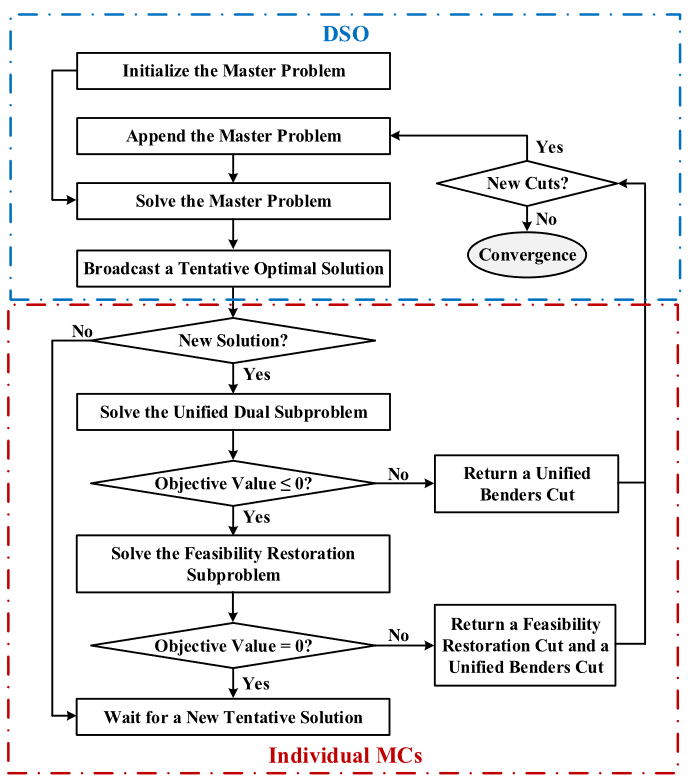
\includegraphics[width=0.8\textwidth]{./pic/IterationProcess.png}
    \caption{迭代过程示意图}
    \label{fig:iteration_process}
\end{figure}


\section{双层问题:小规模模型提取}
仅提取上下层模型中相耦合的变量所涉及到的约束条件, 其余约束省略.
\subsection{上层模型}
\subsubsection{上层目标函数}
以多能互补系统等年值下的系统总投资最小为优化目标:
\setcounter{equation}{0}
\begin{align}
    \min\left(C_{cap}+C_{o\&m}+C_{dep}\right)
\end{align}
式中, $C_{cap}$为系统等年值下的总投资成本, $C_{o\&m}$为系统年运维成本, $C_{dep}$为系统折旧成本.

系统等年值下的总投资成本计算方式如下:
\begin{align}
    C_{cap}=\sum_{k=1}^4C_{cap,k}\cdot\frac{r(1+r)^m}{(1+r)^m-1}
\end{align}
式中, $r$为折现率, $m$为设备的使用年限, $C_{cap,k}$分别为风电、光伏、储能电池逆变器、储能电池装置、光热、储热装置投资成本.
\begin{align}
    \begin{cases}C_{cap,1}=C_W\cdot\lambda_W\\C_{cap,2}=C_V\cdot\lambda_V\\C_{cap,3}=C_B\cdot\lambda_{B_1}+E_B\cdot\lambda_{B_2}\\C_{cap,4}=C_S\cdot\lambda_{S_1}+E_S\cdot\lambda_{S_2}\end{cases}
\end{align}
式中, 所有的$C, E$均为优化变量.

系统运维成本和折旧成本计算方式如下:
\begin{align}
    \begin{cases}C_{o\&m}=C_{cap}\cdot\gamma_o\\C_{dep}=\dfrac{C_{cap}(1-\gamma_r)}m\end{cases}
\end{align}


\subsubsection{上层约束条件}
1. 界约束
\begin{align}
    \begin{cases}0\le C_W\le C_W^{\max}\\0\le C_V\le C_V^{\max}\\0\le C_B\le C_B^{\max}\\0\le E_B\le E_B^{\max}\\0\le C_S\le C_S^{\max}\\0\le E_S\le E_S^{\max}\end{cases}
\end{align}

2. 储能时长约束
\begin{align}
    \begin{cases}E_B=N_B\cdot C_B\\N_B\geq\underline{N}_B\end{cases}
\end{align}

\subsection{下层模型}
\subsubsection{下层目标函数}
以等年值下的系统收益最大为优化目标:
\begin{equation}
    \max I
\end{equation}
\subsubsection{下层约束条件}



\end{document}
